% !TEX encoding = UTF-8 Unicode
\documentclass[9pt, oneside]{extarticle}   	% use for two column: ,twocolumn
\usepackage{hyperref}
\usepackage{fancyvrb}
	\fvset{tabsize=4}%changes tab spacing in verbatim from 8 to 4
%\usepackage{geometry}                		% See geometry.pdf to learn the layout options. There are lots.
%\geometry{letterpaper}                   		% ... or a4paper or a5paper or ... 
%\usepackage[pass,letterpaper]{geometry}
\usepackage[margin=2cm,letterpaper]{geometry}
%\geometry{landscape}                		% Activate for for rotated page geometry
\usepackage[parfill]{parskip}    		% Activate to begin paragraphs with an empty line rather than an indent
\usepackage{graphicx}				% Use pdf, png, jpg, or eps? with pdflatex; use eps in DVI mode
									% TeX will automatically convert eps --> pdf in pdflatex
\usepackage{amssymb}
\usepackage{tikz,adjust box}			%adjustbox is for figures that span 2 columns
\usepackage{dashrule}				%used to make dashed line in text
\usepackage{amsmath}
\usepackage{fancyhdr}				%used to put draft in header
%\pagestyle{fancy}					%
\DeclareMathOperator{\arcsec}{arcsec}	%arcsec, arccsc... not defined inamsmath
\usepackage{exsheets}				%Formats questions and solutions
\SetupExSheets{solution/print=false,question/name={},solution/name={}}		%Solutions on or off; 
\SetupExSheets{headings=runin}		% Puts questions next to number
\SetupExSheets{use-classes={easy,medium,hard}}	% Print questions by difficulty level
\usepackage{natbib,endnotes}			%Bibliography and Footnote to endnote
\usepackage{title sec}				%Format section titles to include horizontal line
%\usepackage{enumitem}				%Allow lists to be a, b, c and not 1, 2, 3
\usepackage{enumerate}
\usepackage{epigraph}
 



%\renewcommand{\theenumi}{\alph{enumi}}
%\setenumerate[0]{label=(\alph*)}
\let\footnote\endnote
\titleformat{\section}
  {\normalfont\Large\bfseries}{\thesection}{1em}{}[{\titlerule[0.8pt]}]
\newcommand{\calc}{\protect\includegraphics[height = 2.5ex]{images/calc.png}}  
%%%%%%%%%%%%%%%%%%%%%%%%%%%%%%%%%%%%%%%%%%%%
%%%%%%%%Convert paragraph to subsubsubsection %%%%%%%%%%%%%%%%
\makeatletter
\renewcommand\paragraph{\@startsection{paragraph}{4}{\z@}%
            {-2.5ex\@plus -1ex \@minus -.25ex}%
            {1.25ex \@plus .25ex}%
            {\normalfont\normalsize\bfseries}}
\makeatother
\setcounter{secnumdepth}{4} % how many sectioning levels to assign numbers to
\setcounter{tocdepth}{4}    % how many sectioning levels to show in ToC
%%%%%%%%%%%%%%%%%%%%%%%%%%%%%%%%%%%%%%%%%%%%%%            

%%%%%%Macros: begin question cntrl command Q or S for solution
%\title{An Introduction to the Tex Document Preparation System}
%\subtitle{Graphs, Diagrams, Presentations and Documents}
%\author{Frank Briody}
%\institute[PHS] % (optional)
% {
%   Prospect High School\\
%   Mt. Prospect, IL
% }
 
% \date[MMC 2019] % (optional)
% {MMC Conference, January 2019}
%\chead{}
\begin{document}

\begin{titlepage} % Suppresses headers and footers on the title page
	\centering % Centre everything on the title page	
	\scshape % Use small caps for all text on the title page
	\vspace*{\baselineskip} % White space at the top of the page
	%------------------------------------------------
	%	Title
	%------------------------------------------------
	\rule{\textwidth}{1.6pt}\vspace*{-\baselineskip}\vspace*{2pt} % Thick horizontal rule
	\rule{\textwidth}{0.4pt} % Thin horizontal rule
	\vspace{0.75\baselineskip} % Whitespace above the title

	{\LARGE AN INTRODUCTION\\TO THE\\[.1in]{\Huge \LaTeX}\\[.1in]DOCUMENT PREPARATION\\SYSTEM} % Title

	\vspace{0.75\baselineskip} % Whitespace below the title
	\rule{\textwidth}{0.4pt}\vspace*{-\baselineskip}\vspace{3.2pt} % Thin horizontal rule
	\rule{\textwidth}{1.6pt} % Thick horizontal rule
	
	\vspace{2\baselineskip} % Whitespace after the title block
	%------------------------------------------------
	%	Subtitle
	%------------------------------------------------
	Graphs, Diagrams, Presentations and Documents % Subtitle or further description
	
	\vspace*{3\baselineskip} % Whitespace under the subtitle
	%------------------------------------------------
	%	Editor(s)
	%------------------------------------------------
	Presented By
	
	\vspace{0.5\baselineskip} % Whitespace before the editors
	{\scshape\Large Frank Briody \\ } % Editor list
	\textit{frankbriody@gmail.com}\\ % 
	\vspace{0.5\baselineskip} % Whitespace below the editor list
	\textit{Prospect High School \\ Mt. Prospect, IL \\ } % Editor affiliation
	
	\includegraphics[width=.1\textwidth]{phs_logo.png}

	\vfill % Whitespace between editor names and publisher logo
	%------------------------------------------------
	%	Publisher
	%------------------------------------------------
	%\plogo % Publisher logo
	\vspace{0.3\baselineskip} % Whitespace under the publisher logo
	2019 % Publication year
	{\large MMC Conference of Workshops}\\[.1in] % Publisher
	\includegraphics[width=\textwidth]{mmc_logo.png}
\end{titlepage}

\tableofcontents
	%\maketitle
\begin{centering}
	\date{\today}
\end{centering}
\newpage
\epigraph{There is only one large computer program I have used in which there are to a decent approximation 0 bugs: Don Knuth's TeX}{\textit{ -- Jaap Weel}}
\section{Pre-Installation} % (fold)
	\label{sec:pre_installation}

	\subsection{What is \LaTeX?} % (fold)
	\label{sub:what_is_la}
	\LaTeX is a macro language used to run \TeX ~commands. Plain text files (.tex) are sent to \TeX ~which returns a .pdf output. Donald Knuth released \TeX ~in 1978 and Leslie Lamport released \LaTeX ~in 1983. \LaTeX ~is free, stable, powerful and well supported. Online versions and installation packages are available for all operating systems.

	\LaTeX ~commands can create standalone formula images, diagrams and graphs that can be inserted into Word or PowerPoint, but can also create entire documents (worksheets or assessments) as well as presentations. Advanced features include bibliographies, animations, data merging, barcodes and pulling information from an external file. 
	% subsection what_is_la (end)
	\subsection{Using \LaTeX ~Inside Schoology, Google Docs, and Other Web-Based Applications} % (fold)
	\label{sub:using_latex}
		Many websites can interpret \LaTeX ~code.  {\bf No installation is required} to perform the following examples where \LaTeX ~code is on the left and the output is shown on the right.  

		\begin{minipage}[t]{2.7in}
			\begin{verbatim}
				m=\frac{y_2-y_1}{x_2-x_1}

				x=\frac{-b\pm\sqrt{b^2-4ac}}{2a}
			\end{verbatim}
		\end{minipage}
		\begin{minipage}[t]{2.7in}
			$m=\frac{y_2-y_1}{x_2-x_1}$\\[.1in]
			$x=\frac{-b\pm\sqrt{b^2-4ac}}{2a}$
			
		\end{minipage}

	Other web-based applications:
		\begin{itemize}
			\item Creating tables: \url{https://www.tablesgenerator.com/}
		 	\item \url{mathb.in} - Creates a temporary URL for sharing a small math document.
		 	\item \url{https://www.codecogs.com/latex/eqneditor.php} - Point and click formula builder that creates \LaTeX ~code.
		 	\item Overleaf - Creates entire \LaTeX ~documents; account (free) required.
		 \end{itemize} 
		 Getting help through a Google search will probably send you to Stack Exchange or Stack Overflow. Look for the green check mark indicating the best answer. For example, search for \texttt{latex document page size}. 
		 
	% subsection using_latex (end)
	% section pre_installation (end)	
\section{Installation} % (fold)
\label{sec:installation}
	\subsection{Download and Install} % (fold)
	\label{sub:download_and_install}
		Search for \texttt{the latex project} and navigate to the \textbf{Get} section. Look in \textbf{\TeX ~Distributions} for your operating system. Do not use \LaTeX3 as it is still in development (as of January 2019). Since the installer is more than 3 gigabytes, it is probably best to download using a wired connection. Note that older versions are available if your operating system is not the current version. (Note to Mac users: In the past Chrome had issues with download failures. Try Safari instead.)

		The installation page (McTex for Mac and probably Tex Live for Windows and Linux) should include both installers and help documents. Running the installer puts the \TeX ~code in the appropriate places, installs necessary fonts and includes at least 2 helper applications. The first is a code editor (TexShop for Mac) and a \TeX ~update tool (Tex Live Utility). Reading the  help documents from the downloads web page, especially any introductions to \LaTeX, ~would be very beneficial. \LaTeX ~has a very steep learning curve but a lot of tutorials, support documents and learning communities are available. YouTube is also a great resource for help with installing and using \LaTeX. 
	% subsection download_and_install (end)
	\subsection{Using a Code Editor} % (fold)
	\label{sub:using_a_code_editor}
		After installation, open the code editor and try running some sample code. For example:
		\begin{verbatim}
		\documentclass{standalone}
		\begin{document}
			$x=\frac{-b\pm\sqrt{b^2-4ac}}{2a}$\\
			$\lim \limits_{x\to18}\frac{2x}{7}$
		\end{document}
		  \end{verbatim}  
		  If you see a pdf with two math statements you have successfully installed \TeX. Explore the different menu options as they may help you learn \LaTeX ~commands. The LaTeX Panel and Matrix Panel under the Window menu can be especially helpful if you are using TeXShop. During the .pdf creation process, \LaTeX ~creates other auxiliary files. While these files are not necessary and can be moved to the trash, the next time a .tex file is compiled they will be regenerated. If your \TeX ~installation was successful, checking for updates would be the next step. 
	% subsection using_a_code_editor (end)
	\subsection{Updating} % (fold)
	\label{sub:updating}
		\TeX ~has many sub-programs called packages that are installed but do not run unless called. (As of 2012, the number of packages was near 2,500.) Calling packages only when needed allows \LaTeX ~to execute quickly but also offer thousands of specific uses. Trusted packages are stored at CTAN (The Comprehensive \TeX ~Archive Network) and can be updated by using the \TeX ~Live Utility (Mac) program included in the installation.  One of \LaTeX's attractive features is its stability. In general, updates do not break existing code. To update your packages, open the update program and choose update. (Note that the \TeX ~Live Utility program itself is also occasionally updated so you may be prompted to update \TeX ~Live Utility before you can use \TeX ~Live Utility to update your computer's \TeX ~installation.) As the program runs, you should see the list of packages that are being updated, installed or removed.  	  
	% subsection updating (end)	  
	\subsection{Optional Installations} % (fold)
	\label{sub:optional_installations}
		Once you have been using \LaTeX ~for a while, you may want to consider some additional installations.
		\begin{itemize}
			\item \textbf{Skim} - Skim is a free pdf viewer that integrates well with \LaTeX. After setting a preference in Skim, you can click on a specific place in the pdf output and be taken to the corresponding code in your code editor. Skim can also be used as a slide show viewer when making \LaTeX ~to Beamer presentations. Skim cannot display Beamer animations but Adobe Acrobat can.
			\item \textbf{Sublime Text 3} - Sublime Text is a popular code editor that also offers some optional \LaTeX ~customizations. The \LaTeX Tools and \LaTeX-cwl plugins for Sublime Text make writing code much more efficient. Autocompletion of common commands and document navigation are two examples. Sublime Text is not free but does allow for an unlimited free trial. 
			\item \textbf{TextExpander} - Since many \LaTeX ~commands are repeated, TextExpander can store store and paste commonly used lines of code. Variables can be used inside snippets. When a snippet is summoned from TextExpander, the values for the variable are input before the code is pasted into the .tex document. 
		\end{itemize}
	% subsection optional_installations (end)
		  
	
% section installation (end)
\section{Diagrams and Graphs} % (fold)
\label{sec:diagrams_and_graphs}
	\LaTeX ~documents can include diagrams two different ways. The first is by using an existing image file (.png, .jpg or .pdf) and the second is by generating an image using either the \texttt{TikZ} or \texttt{PSTricks} packages. (Only the \texttt{TikZ} package will be discussed here.) Again, well organized manuals exist for each as well as tutorials and videos. 
		\begin{itemize}
			\item \url{https://cremeronline.com/LaTeX/minimaltikz.pdf}
			\item \url{http://www.math.uni-leipzig.de/~hellmund/LaTeX/pgf-tut.pdf}
		\end{itemize}
	
	\subsection{Inserting an Image} % (fold)
	\label{sub:insert_image_grids}
	To insert an image, put the file in the same directory (folder) as your .tex file and use the following code:
	\begin{Verbatim}
\includegraphics[width=\textwidth]{mmc_logo.png}\\	 
	 \end{Verbatim} 
	 The \verb|width=\textwidth| scales the image to match the width of the current page, column, or frame. To reduce the size, insert a proportion value in front of the \verb|\textwidth| command. For example, \verb|width=.4\textwidth| will scale the image to 40\% of the available width. Add \verb|\centering| if you would like to image horizontally centered in the available space.
	\subsection{Blank Grids} % (fold)
	\label{sub:blank_grids}
		\subsubsection{Number Line}
		\begin{minipage}[t]{2.7in}
\begin{Verbatim}
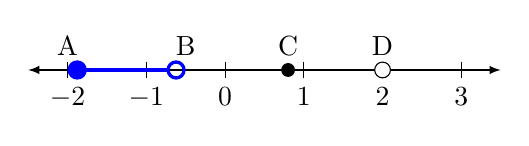
\begin{tikzpicture}[scale=1.0]
\usetikzlibrary{arrows}
  \draw[latex-latex] (-2.5,0) -- (3.5,0);
    \foreach \x in  {-2,-1,0,1,2,3} 
      \draw[shift={(\x,0)},color=black] (0pt,3pt) -- (0pt,-3pt);
    \foreach \x in {-2,-1,0,1,2,3} 
      \draw[shift={(\x,0)},color=black] (0pt,0pt) -- (0pt,-3pt) node[below] {$\x$};
    \draw[very thick,*-o,blue] (-2,0) -- (-.5,0);
    \node at (-2,.3) {A};
    \node at (-.5,.3) {B};
    \fill (0.8,0)  circle[radius=2.5pt];
    \node at (0.8,.3) {C};
    \draw[fill=white] (2,0) circle (.1cm);
    \node at (2,.3) {D};
\end{tikzpicture}
\end{Verbatim}
		\end{minipage}
		\begin{minipage}[c]{2.7in}
			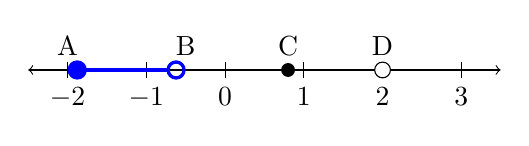
\begin{tikzpicture}[scale=1.0]
			\usetikzlibrary{arrows}
			\draw[<->] (-2.5,0) -- (3.5,0); %edit here for the axis
			\foreach \x in  {-2,-1,0,1,2,3} % edit here for the vertical lines
			\draw[shift={(\x,0)},color=black] (0pt,3pt) -- (0pt,-3pt);
			\foreach \x in {-2,-1,0,1,2,3} % edit here for the numbers
			\draw[shift={(\x,0)},color=black] (0pt,0pt) -- (0pt,-3pt) node[below]
			{$\x$};
			\draw[very thick,*-o,blue] (-2,0) -- (-.5,0);
			\node at (-2,.3) {A};
			\node at (-.5,.3) {B};
			\fill (0.8,0)  circle[radius=2.5pt];
			\node at (0.8,.3) {C};
			\draw[fill=white] (2,0) circle (.1cm);
			\node at (2,.3) {D};
			\end{tikzpicture}
		\end{minipage}
		\subsubsection{Cartesian Plane}
			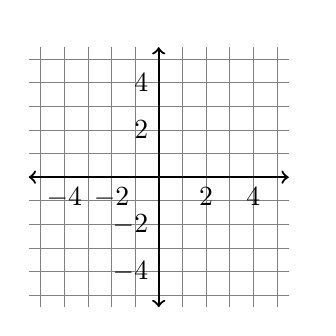
\begin{tikzpicture}[xscale=.3,yscale=.3]%[y=1cm,x=1cm]
			\draw[style = help lines, step=1cm] (-5.5,-5.5) grid (5.5,5.5);
			 \draw[thick,<->] (-5.5,0) -- (5.5,0) node[anchor=north west] {};%{x};
			 \draw[thick,<->] (0,-5.5) -- (0,5.5) node[anchor=south east] {};%{y};
			 \foreach \x in {-4,-2,2,4}
			 \draw (\x cm,1pt) -- (\x cm,-1pt) node[anchor=north] {$\x$};
			 \foreach \y in {-4, -2, 2,4}
			 \draw (1pt,\y cm) -- (-1pt,\y cm) node[anchor=east] {$\y$};
			 %\draw[ultra thick,blue,<->] plot[domain=-3.89:3.75,samples=100] (\x,{.2*(\x+2)^2*(\x-3)});
			 %\draw[ultra thick,blue,-] (-3,-4) -- (2,4);
			 %\draw [red,ultra thick,domain=0:180] plot ({3*cos(\x)+2}, {3*sin(\x)});
            %\draw[ultra thick, blue,] (-2,-4) to [out=0, in=180] (4,1);
            %\draw[ultra thick, blue,] (0,-3) -- (1,0) .. controls (2.5,4) and (2.5,0) .. (3,0) .. controls (4.5,.9) .. (6,3);
            %\foreach\x/\y/\z in {-1.8/1.2/P,-1/.3/Q,3.2/3.8/R,6.5/5/S,7.6/6/T}			 
               %? \draw [fill=black] (\x,\y)circle (3pt) node[above] {\z};
		\end{tikzpicture}
			\begin{verbatim}
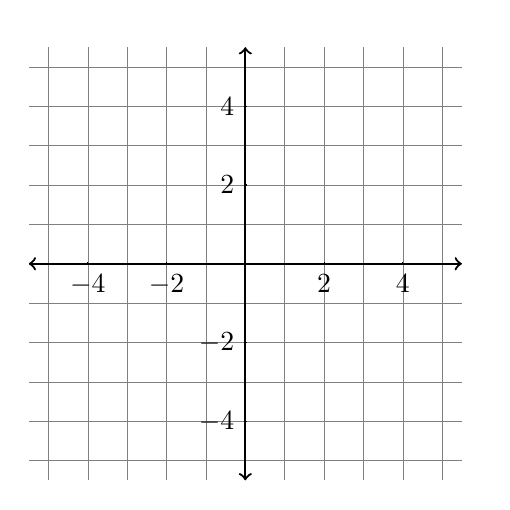
\begin{tikzpicture}[xscale=.5,yscale=.5]
     \draw[style = help lines, step=1cm] (-5.5,-5.5) grid (5.5,5.5);
     \draw[thick,<->] (-5.5,0) -- (5.5,0) node[anchor=north west] {};
     \draw[thick,<->] (0,-5.5) -- (0,5.5) node[anchor=south east] {};
     \foreach \x in {-4,-2,2,4}
          \draw (\x cm,1pt) -- (\x cm,-1pt) node[anchor=north] {$\x$};
     \foreach \y in {-4, -2, 2,4}
           \draw (1pt,\y cm) -- (-1pt,\y cm) node[anchor=east] {$\y$};
\end{tikzpicture}
			\end{verbatim}
	% subsection blank_grids (end)
	\subsection{Functions} % (fold)
	\label{sub:functions}
		\subsubsection[Basic]{Functions, Points and Piecewise}
	Function, point (left)
	\begin{verbatim}
	\draw[ultra thick,blue,<->] plot[domain=-3.89:3.75,samples=100] 
	     (\x,{.2*(\x+2)^2*(\x-3)});
	\fill (1.33,-3.7)  circle[radius=5pt] node[anchor=north west]{P};
	\end{verbatim}
	Points, dashed line, piecewise (right)
	\begin{verbatim}
	\foreach\x/\y/\z in {-4/2/P,-3/-1/Q,-2/-2/R,-1/-1/S,0/2/T}			 
     \draw [fill=black] (\x,\y)circle (3pt) node[below left] {\z};
	\draw[dashed,<->] plot[domain=-4.5:0.5,samples=100] (\x,{(\x+2)^2-2)});   
	\draw[->,ultra thick,blue] (-1,-4) -- (4,1);
	\end{verbatim}
	\begin{minipage}[c]{2.7in}
		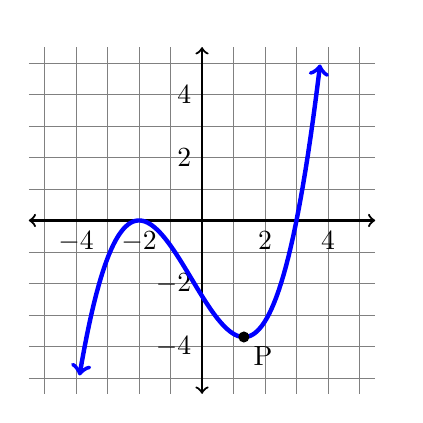
\begin{tikzpicture}[xscale=.4,yscale=.4]%[y=1cm,x=1cm]
			\draw[style = help lines, step=1cm] (-5.5,-5.5) grid (5.5,5.5);
			 \draw[thick,<->] (-5.5,0) -- (5.5,0) node[anchor=north west] {};%{x};
			 \draw[thick,<->] (0,-5.5) -- (0,5.5) node[anchor=south east] {};%{y};
			 \foreach \x in {-4,-2,2,4}
			 \draw (\x cm,1pt) -- (\x cm,-1pt) node[anchor=north] {$\x$};
			 \foreach \y in {-4, -2, 2,4}
			 \draw (1pt,\y cm) -- (-1pt,\y cm) node[anchor=east] {$\y$};
			 \draw[ultra thick,blue,<->] plot[domain=-3.89:3.75,samples=100] (\x,{.2*(\x+2)^2*(\x-3)});
			 \fill (1.33,-3.7)  circle[radius=5pt] node[anchor=north west]{P};
			 %\draw[ultra thick,blue,-] (-3,-4) -- (2,4);
			 %\draw [red,ultra thick,domain=0:180] plot ({3*cos(\x)+2}, {3*sin(\x)});
            %\draw[ultra thick, blue,] (-2,-4) to [out=0, in=180] (4,1);
            %\draw[ultra thick, blue,] (0,-3) -- (1,0) .. controls (2.5,4) and (2.5,0) .. (3,0) .. controls (4.5,.9) .. (6,3);
            %\foreach\x/\y/\z in {-1.8/1.2/P,-1/.3/Q,3.2/3.8/R,6.5/5/S,7.6/6/T}			 
               %? \draw [fill=black] (\x,\y)circle (3pt) node[above] {\z};
         \end{tikzpicture}
	\end{minipage}
	\begin{minipage}[c]{2.7in}
		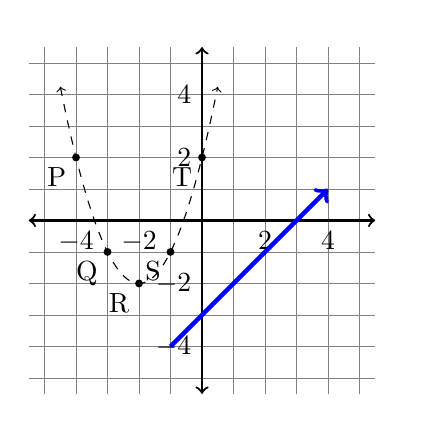
\begin{tikzpicture}[xscale=.4,yscale=.4]%[y=1cm,x=1cm]
			\usetikzlibrary{arrows}
			\draw[style = help lines, step=1cm] (-5.5,-5.5) grid (5.5,5.5);
			 \draw[thick,<->] (-5.5,0) -- (5.5,0) node[anchor=north west] {};%{x};
			 \draw[thick,<->] (0,-5.5) -- (0,5.5) node[anchor=south east] {};%{y};
			 \foreach \x in {-4,-2,2,4}
			 \draw (\x cm,1pt) -- (\x cm,-1pt) node[anchor=north] {$\x$};
			 \foreach \y in {-4, -2, 2,4}
			 \draw (1pt,\y cm) -- (-1pt,\y cm) node[anchor=east] {$\y$};
			 %\draw[ultra thick,blue,<->] plot[domain=-3.89:3.75,samples=100] (\x,{.2*(\x+2)^2*(\x-3)});
			 \draw[->,ultra thick,blue] (-1,-4) -- (4,1);
			 %\draw [red,ultra thick,domain=0:180] plot ({3*cos(\x)+2}, {3*sin(\x)});
            %\draw[ultra thick, blue,] (-2,-4) to [out=0, in=180] (4,1);
            %\draw[ultra thick, blue,] (0,-3) -- (1,0) .. controls (2.5,4) and (2.5,0) .. (3,0) .. controls (4.5,.9) .. (6,3);
            \foreach\x/\y/\z in {-4/2/P,-3/-1/Q,-2/-2/R,-1/-1/S,0/2/T}			 
                \draw [fill=black] (\x,\y)circle (3pt) node[below left] {\z};
            \draw[dashed,<->] plot[domain=-4.5:0.5,samples=100] (\x,{(\x+2)^2-2)});   
         \end{tikzpicture}
         \end{minipage}
         \subsubsection[Scale]{Changing Scale}
		\begin{verbatim}
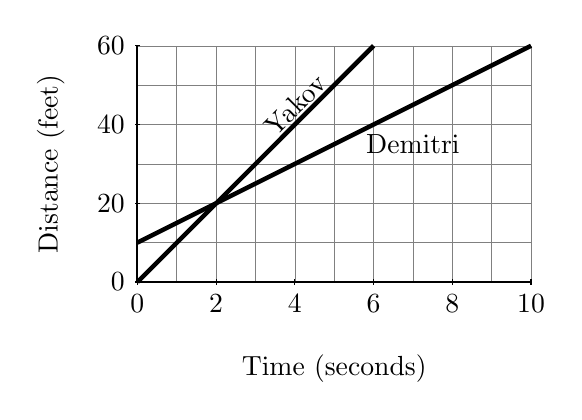
\begin{tikzpicture}[y=.05cm, x=.5cm]   
    \draw[style=help lines, ystep=10, xstep=1] (0,0) grid (10,60);
    \draw[thick,-] (0,0) -- coordinate (x axis mid) (10,0);
    \draw[thick,-] (0,0) -- coordinate (y axis mid) (0,60);
    \foreach \x in {0,2,4,6,8,10}
        \draw (\x ,1pt) -- (\x ,-1pt) node[anchor=north] {$\x$};
    \foreach \y in {0,20,40,60}
        \draw (1pt,\y ) -- (-1pt,\y ) node[anchor=east] {$\y$};
    \draw[-, ultra thick, domain=-0:6,smooth] plot (\x, {10*\x}); 
    \node[rotate=45] at (4,45) {Yakov};
    \node[rotate=0] at (7,35) {Demitri};
    \draw[-, ultra thick, domain=-0:10,smooth] plot (\x, {5*\x+10});
    \node[below=0.8cm] at (x axis mid) {Time (seconds)};
    \node[rotate=90, above=0.8cm] at (y axis mid) {Distance (feet)};
\end{tikzpicture}\\
		\end{verbatim}

		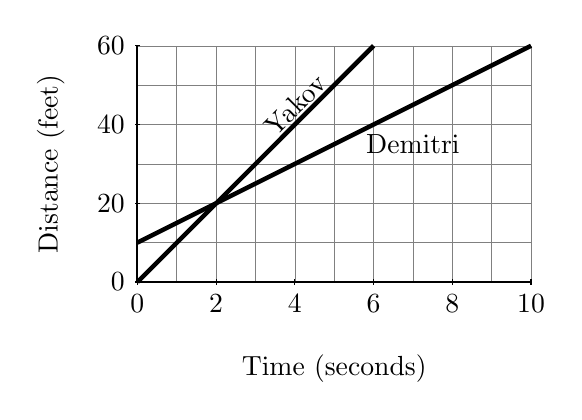
\begin{tikzpicture}[y=.05cm, x=.5cm]
			\draw[style=help lines, ystep=10, xstep=1] (0,0) grid (10,60);
			\draw[thick,-] (0,0) -- coordinate (x axis mid) (10,0);
			\draw[thick,-] (0,0) -- coordinate (y axis mid) (0,60);
			\foreach \x in {0,2,4,6,8,10}
			    \draw (\x ,1pt) -- (\x ,-1pt) node[anchor=north] {$\x$};
			\foreach \y in {0,20,40,60}
			    \draw (1pt,\y ) -- (-1pt,\y ) node[anchor=east] {$\y$};
			\draw[-, ultra thick, domain=-0:6,smooth] plot (\x, {10*\x}); 
			\node[rotate=45] at (4,45) {Yakov};
			\node[rotate=0] at (7,35) {Demitri};
			\draw[-, ultra thick, domain=-0:10,smooth] plot (\x, {5*\x+10}); 
			\node[below=0.8cm] at (x axis mid) {Time (seconds)};
			\node[rotate=90, above=0.8cm] at (y axis mid) {Distance (feet)};
			\end{tikzpicture}

		\subsubsection[Domain]{Rational and Setting Domain}
			Use Desmos to find precise domain values. Adding a caption to a graph is also possible by using the \texttt{figure} and \texttt{caption} commands. (Putting information inside a node is usually a more efficient use of space.)
				\begin{Verbatim}
\begin{figure}[h]
	\begin{centering}
		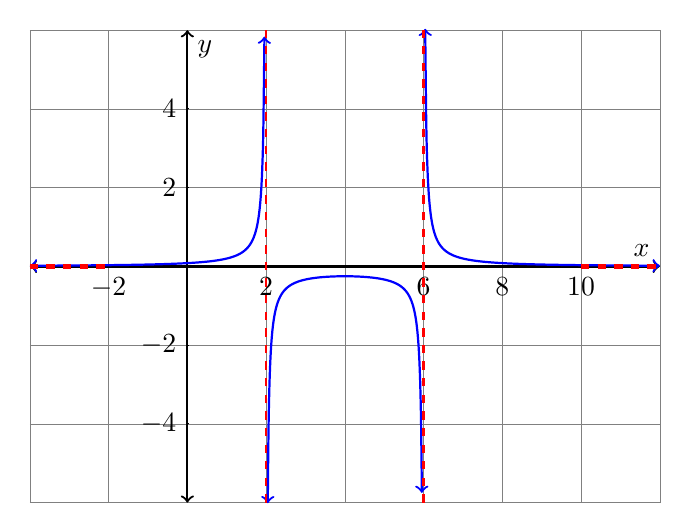
\begin{tikzpicture}[scale=.5]\label{caption_ex}
			\draw[style=help lines, ystep=2, xstep=2] (-4,-6) grid (12,6);%grid
			\draw[thick,<->] (-4,0) -- (12,0) node[anchor=south east] {$x$};
			\draw[thick,<->] (0,-6) -- (0,6) node[anchor=north west] {$y$};
			\foreach \x in {-2,2,6,8,10}
			    \draw (\x cm,1pt) -- (\x cm,-1pt) node[anchor=north] {$\x$};
			\foreach \y in {-4,-2,2,4}
			    \draw (1pt,\y cm) -- (-1pt,\y cm) node[anchor=east] {$\y$};
			%\draw[<->, ultra thick, domain=0:8,smooth] plot (\x, {\x*\x-8*\x+12});
			\draw[blue,<->, thick, domain=-4:1.959,smooth,samples=200] plot (\x, {1/(\x*\x-8*\x+12)});
			\draw[blue,<->, thick, domain=2.042:5.958,smooth,samples=200] plot (\x, {1/(\x*\x-8*\x+12)});
			\draw[blue,<->, thick, domain=6.041:12,smooth,samples=200] plot (\x, {1/(\x*\x-8*\x+12)});
			\draw[red,thick,dashed] (2,-6) -- (2,6);%Vert Asymp
			\draw[red,thick,dashed] (6,-6) -- (6,6);%Vert Asymp
			\draw[red,ultra thick,dashed] (-4,0) -- (-2,0);%Horiz Asymp
			\draw[red,ultra thick,dashed] (10,0) -- (12,0);%Horiz Asymp
		\end{tikzpicture}
		\caption{$f(x)=\frac{1}{x^2-8x+12}$}\label{fig: f1}
	\end{centering}
\end{figure}
				\end{Verbatim}
		
				\begin{figure}[h]
					\begin{centering}
						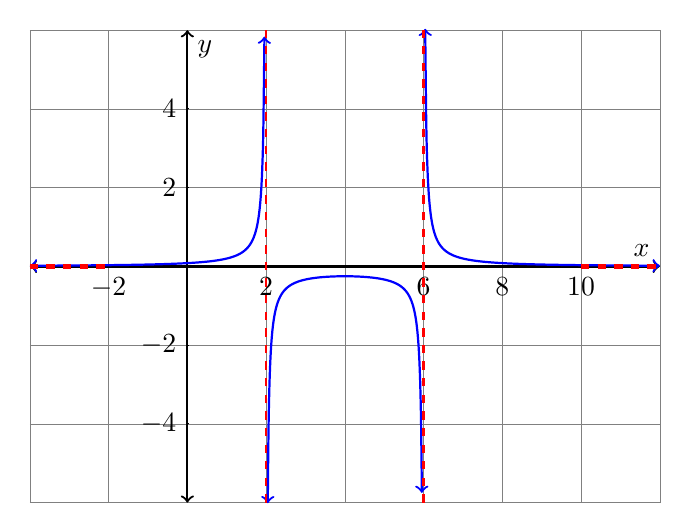
\begin{tikzpicture}[scale=.5]\label{caption_ex}
							\draw[style=help lines, ystep=2, xstep=2] (-4,-6) grid (12,6);%grid
							\draw[thick,<->] (-4,0) -- (12,0) node[anchor=south east] {$x$};
							\draw[thick,<->] (0,-6) -- (0,6) node[anchor=north west] {$y$};
							\foreach \x in {-2,2,6,8,10}
							    \draw (\x cm,1pt) -- (\x cm,-1pt) node[anchor=north] {$\x$};
							\foreach \y in {-4,-2,2,4}
							    \draw (1pt,\y cm) -- (-1pt,\y cm) node[anchor=east] {$\y$};
							%\draw[<->, ultra thick, domain=0:8,smooth] plot (\x, {\x*\x-8*\x+12});
							\draw[blue,<->, thick, domain=-4:1.959,smooth,samples=200] plot (\x, {1/(\x*\x-8*\x+12)});
							\draw[blue,<->, thick, domain=2.042:5.958,smooth,samples=200] plot (\x, {1/(\x*\x-8*\x+12)});
							\draw[blue,<->, thick, domain=6.041:12,smooth,samples=200] plot (\x, {1/(\x*\x-8*\x+12)});
							\draw[red,thick,dashed] (2,-6) -- (2,6);%Vert Asymp
							\draw[red,thick,dashed] (6,-6) -- (6,6);%Vert Asymp
							\draw[red,ultra thick,dashed] (-4,0) -- (-2,0);%Horiz Asymp
							\draw[red,ultra thick,dashed] (10,0) -- (12,0);%Horiz Asymp
						\end{tikzpicture}
						\caption{$f(x)=\frac{1}{x^2-8x+12}$}\label{fig: f1}
					\end{centering}
				\end{figure}
	\subsubsection[Drawing]{Drawing Curves}
	The TikZ package has extensive drawing capabilities. Lines, arcs and shading can be used to create functions, relations and other mathematical or scientific diagrams. The TikZ manual \href{https://www.bu.edu/math/files/2013/08/tikzpgfmanual.pdf}{https://www.bu.edu/math/files/2013/08/tikzpgfmanual.pdf} contains enough examples that could help produce just about any two- or three-dimensional diagram.  
		\begin{Verbatim}
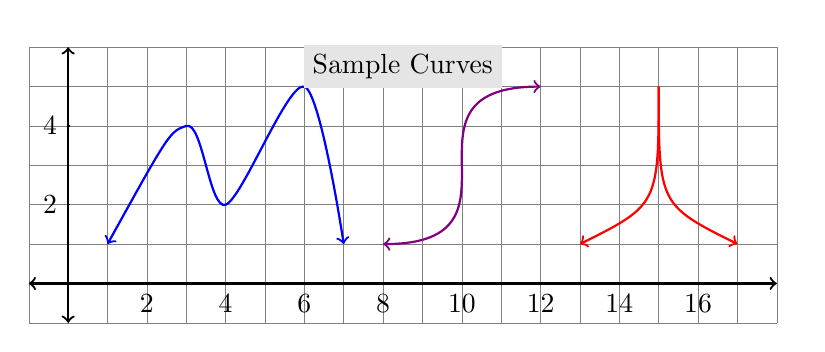
\begin{tikzpicture}[xscale=.5,yscale=.5]\label{node_ex}%[y=1cm,x=1cm]
	\draw[style = help lines, step=1cm] (-1,-1) grid (18,6);
	\foreach \x in {2,4,6,8,10,12,14,16}
		\draw (\x cm,1pt) -- (\x cm,-1pt) node[anchor=north] {$\x$};
	\foreach \y in {2,4}
		\draw (1pt,\y cm) -- (-1pt,\y cm) node[anchor=east] {$\y$};
	\draw[thick,<->] (-1,0) -- (18,0) node[anchor=north west] {};%{x};
	\draw[thick,<->] (0,-1) -- (0,6) node[anchor=south east] {};%{y};
	\draw[blue,<->,thick] plot [smooth] coordinates {(1,1) (3,4) (4,2) (6,5) (7,1)};
	\draw[violet, thick,<->] (8,1) .. controls (12,1) and (8,5) .. (12,5);
	\draw[red, thick,<-] (13,1) .. controls (15,2) .. (15,5);
	\draw[red, thick,->] (15,5) .. controls (15,2) .. (17,1);
	\node[fill=black!10] at (8.5,5.5) {Sample Curves};						
\end{tikzpicture}\\                     
		\end{Verbatim}
		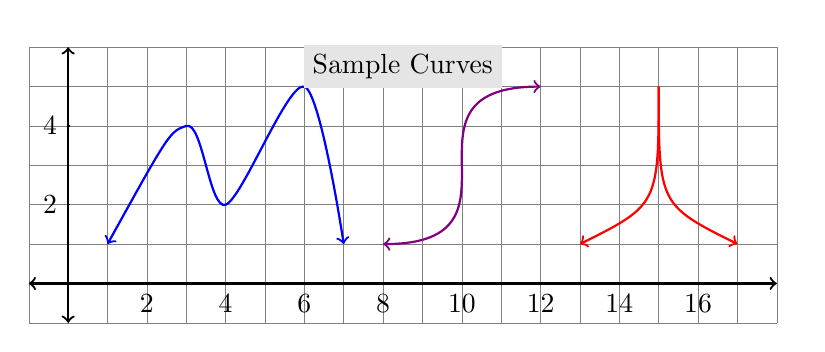
\begin{tikzpicture}[xscale=.5,yscale=.5]\label{node_ex}%[y=1cm,x=1cm]
            \draw[style = help lines, step=1cm] (-1,-1) grid (18,6);
            \foreach \x in {2,4,6,8,10,12,14,16}
	            \draw (\x cm,1pt) -- (\x cm,-1pt) node[anchor=north] {$\x$};
            \foreach \y in {2,4}
               \draw (1pt,\y cm) -- (-1pt,\y cm) node[anchor=east] {$\y$};
            \draw[thick,<->] (-1,0) -- (18,0) node[anchor=north west] {};%{x};
            \draw[thick,<->] (0,-1) -- (0,6) node[anchor=south east] {};%{y};
			\draw[blue,<->,thick] plot [smooth] coordinates {(1,1) (3,4) (4,2) (6,5) (7,1)};
			\draw[violet, thick,<->] (8,1) .. controls (12,1) and (8,5) .. (12,5);
			\draw[red, thick,<-] (13,1) .. controls (15,2) .. (15,5);
			\draw[red, thick,->] (15,5) .. controls (15,2) .. (17,1);
			\node[fill=black!10] at (8.5,5.5) {Sample Curves};			
        \end{tikzpicture}\\                     
		\subsubsection[Legend]{Adding a Legend}
		Putting a name on a figure can be accomplished in one of three ways:
		\begin{enumerate}
		\item Using a caption like \ref{caption_ex}.
		\item Using a node like \ref{node_ex}.
		\item Creating a legend (below). 
		\end{enumerate}
			\begin{Verbatim}
\node[draw=black,thick,fill=black!10,rounded corners=2pt,below left=2mm] at (10,-1) {%
	\begin{tabular}{@{}r@{ }l@{}}
	\raisebox{2pt}{\tikz{\draw[thick,blue] (0,0) -- (5mm,0);}}&$y=\log_2 x$\\
	\raisebox{2pt}{\tikz{\draw[thick,green] (0,0) -- (5mm,0);}}&$y=\log_4 x$\\
	\raisebox{2pt}{\tikz{\draw[thick,red] (0,0) -- (5mm,0);}}&$y=\log_5 x$\\
	\raisebox{2pt}{\tikz{\draw[thick,orange] (0,0) -- (5mm,0);}}&$y=\log_{10} x$\\
	\raisebox{2pt}{\tikz{\draw[thick,brown] (0,0) -- (5mm,0);}}&$y=\log_{e} x=\ln x$
\end{tabular}};
			\end{Verbatim}
			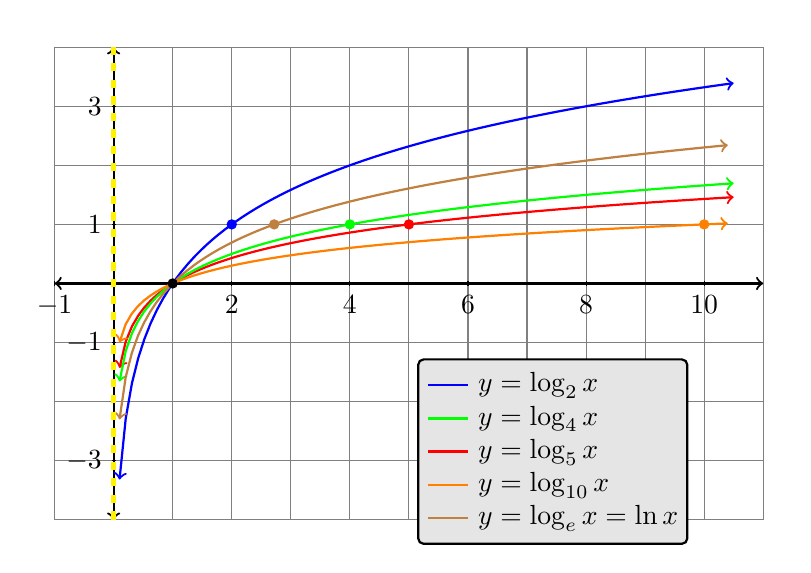
\begin{tikzpicture}[scale=.75]
				\draw[step=1cm,gray, thin] (-1,-4) grid (11,4);
				\draw[thick,<->] (-1,0) -- (11,0) node[anchor=north west] {};%{x};
				\draw[thick,<->] (0,-4) -- (0,4) node[anchor=south east] {};%{y};
				\foreach \x in {-1,2,4, 6, 8, 10}
				\draw (\x cm,1pt) -- (\x cm,-1pt) node[anchor=north] {$\x$};
				\foreach \y in {-1,-3,1,3}
				\draw (1pt,\y cm) -- (-1pt,\y cm) node[anchor=east] {$\y$};
				\draw[<->,thick,blue] plot[domain=0.1:10.5,samples=100] (\x,{log2(\x)});
				\draw[<->,thick,red] plot[domain=0.1:10.5,samples=100] (\x,{(log2(\x))/(log2(5))});
				\draw[<->,thick,green] plot[domain=0.1:10.5,samples=100] (\x,{(log2(\x))/(log2(4))});
				\draw[<->,thick,orange] plot[domain=0.1:10.4,samples=100] (\x,{(log2(\x))/(log2(10))});
				\draw[<->,thick,brown] plot[domain=0.1:10.4,samples=100] (\x,{(log2(\x))/(log2(2.718))});
				\draw[ultra thick, dashed,yellow] (0,-4)--(0,4);
				\fill (1,0) circle[radius=2.5pt];
				\fill[blue] (2,1) circle[radius=2.5pt];
				\fill[red] (5,1) circle[radius=2.5pt];
				\fill[green] (4,1) circle[radius=2.5pt];
				\fill[orange] (10,1) circle[radius=2.5pt];
				\fill[brown] (2.71828,1) circle[radius=2.5pt];
				%\node[draw=black,thick,fill=white,rounded corners=2pt,below left=2mm] at (3.6,4.2) {%
				\node[draw=black,thick,fill=black!10,rounded corners=2pt,below left=2mm] at (10,-1) {%
				\begin{tabular}{@{}r@{ }l@{}}
				 \raisebox{2pt}{\tikz{\draw[thick,blue] (0,0) -- (5mm,0);}}&$y=\log_2 x$\\
				 \raisebox{2pt}{\tikz{\draw[thick,green] (0,0) -- (5mm,0);}}&$y=\log_4 x$\\
				 \raisebox{2pt}{\tikz{\draw[thick,red] (0,0) -- (5mm,0);}}&$y=\log_5 x$\\
				 \raisebox{2pt}{\tikz{\draw[thick,orange] (0,0) -- (5mm,0);}}&$y=\log_{10} x$\\
				 \raisebox{2pt}{\tikz{\draw[thick,brown] (0,0) -- (5mm,0);}}&$y=\log_{e} x=\ln x$
				\end{tabular}};
			\end{tikzpicture}

		\subsubsection[Gallery]{The Tikz Gallery of Examples}
		There is a huge Tikz gallery of examples at \url{http://www.texample.net/tikz/examples/}. In the \texttt{Scientific and technical areas} section there is a \texttt{Mathematics} tag. Find a usable diagram, copy and paste the code then modify as needed. Graph paper, polar coordinate and unit circle examples are available.  
			
	% subsection functions (end)
	\subsection{Diagrams} % (fold)
	\label{sub:diagrams}
	A simple diagram:\\
		\begin{minipage}[T]{.35\textwidth}
			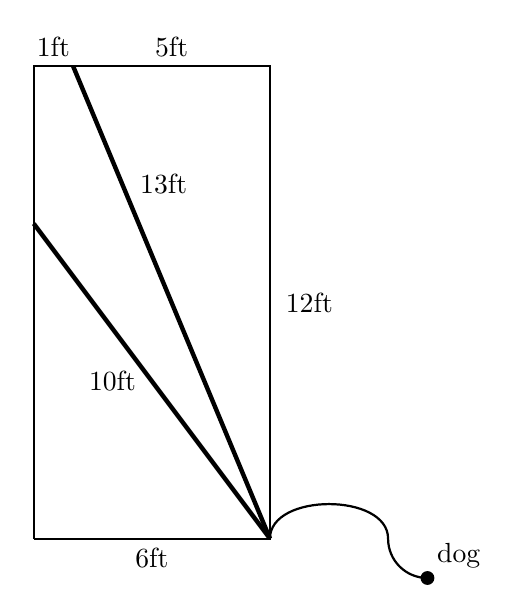
\begin{tikzpicture}[scale=.5]
			%\draw[gray] (0,-2) grid (10,12);
			\draw[  thick,-] (0,0) -- (6,0) -- (6,12)--(0,12)--(0,0);%node[anchor=north east] {m};
			\draw[ultra thick,-] (6,0)--(0,8);
			\draw[ultra thick,-] (6,0)--(1,12);
			%\node[anchor=north east] {m};
			\node at (.5,12.5) {1ft};
			\node at (3.5,12.5) {5ft};
			\node at (7,6) {12ft};
			\node at (3,-.5) {6ft};
			\node at (3.3,9) {13ft};
			\node at (2,4) {10ft};
			\fill (10,-1)  circle[radius=5pt] node[anchor=south west]  {dog};
			\draw [-,thick] (6,0) [out=90 ,in=90] to (9,0) [out=270 ,in=180 ] to (10,-1);
			\end{tikzpicture}
		\end{minipage}
		\begin{minipage}[T]{.65\textwidth}
			\begin{Verbatim}
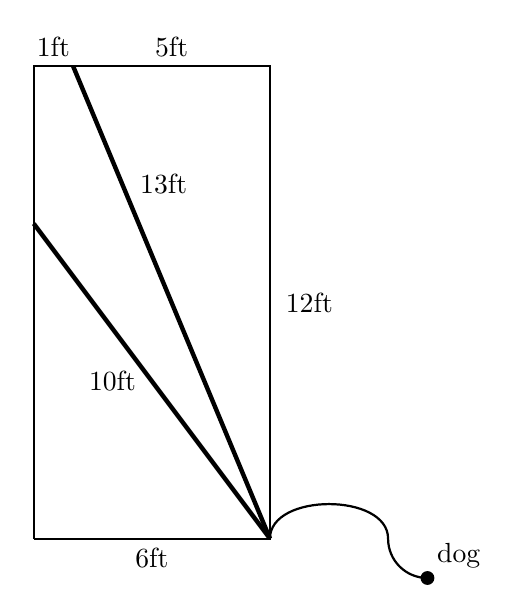
\begin{tikzpicture}[scale=.5]
	%\draw[gray] (0,-2) grid (10,12);
	\draw[  thick,-] (0,0) -- (6,0) -- (6,12)--(0,12)--(0,0);
	\draw[ultra thick,-] (6,0)--(0,8);
	\draw[ultra thick,-] (6,0)--(1,12);
	\node at (.5,12.5) {1ft};
	\node at (3.5,12.5) {5ft};
	\node at (7,6) {12ft};
	\node at (3,-.5) {6ft};
	\node at (3.3,9) {13ft};
	\node at (2,4) {10ft};
	\fill (10,-1)  circle[radius=5pt] node[anchor=south west]  {dog};
	\draw [-,thick] (6,0) [out=90 ,in=90] to (9,0) [out=270 ,in=180 ] 
		to (10,-1);
\end{tikzpicture}
			\end{Verbatim}
		\end{minipage}

\quad\\

	A more involved example:\\
		\begin{minipage}[T]{.55\textwidth}
			A man (M) standing on the beach throws a ball (B) into the water 20 feet down the shoreline and 6 feet into the water (see diagram). Elvis the dog runs up the shoreline and then jumps into the water at S to swim out to the ball. If Elvis can run $10$ft/sec and swim at $4$ft/sec write an expression for the time it takes Elvis to get to the ball as a function of $x$ where $x$ is the distance Elvis runs on the beach (M to S). ({\bf NOTE}: You only need to set up the function. {\bf DO NOT} simplify or find the maximum or minimum.)
		\end{minipage}
		\begin{minipage}[T]{.05\textwidth}
		\quad\\
		\end{minipage}
		\begin{minipage}[T]{.35\textwidth}
		                \usetikzlibrary{calc}
		            \newcommand\irregularline[2]{%
		                let \n1 = {rand*(#1)} in
		                +(0,\n1)
		                \foreach \a in {0.1,0.2,...,#2}{
		                let \n1 = {rand*(#1)} in
		                -- +(\a,\n1)
		                    } 
		            } 
		 \begin{tikzpicture}[scale=.5]
		            \draw[thick,blue] (-6,4) \irregularline{0.1cm}{12};
		            \fill[gray,opacity=.5] (-6,0) rectangle (6,4);
		            \draw[|-|] (-5,0)--(-5,4) node [midway] {6ft};
		            \draw[thick,dashed] (-4,0)--(-4,4);
		            \draw[<-,ultra thick,dashed] (-4,0)--(-1,4);
		            \draw[<-,ultra thick,dashed] (-1,4.2)--(5,4.2);
		            \draw[|-|] (-4,6)--(5,6) node [midway,fill=white] {20ft};
		            \node[anchor=south] at (-4,4) {$O$};
		            \node[anchor=north west] at (-4,0) {$B$};
		            \node[anchor=north west] at (-1,4) {$S$};
		            \node[anchor=north west] at (5,4) {$M$};
		            \draw[fill=black] (-4,0) circle (5pt);%CLOSED CIRCLE
		            \draw[fill=black] (-1,4.1) circle (5pt);%CLOSED CIRCLE
		            \draw[fill=black] (5,4.1) circle (5pt);%CLOSED CIRCLE
		            \draw (-4,4)--(-3.5,4)--(-3.5,3.5)--(-4,3.5)--(-4,4);
		            \end{tikzpicture}
		\end{minipage}
	
\begin{Verbatim}
\usetikzlibrary{calc}
	\newcommand\irregularline[2]{%
	    let \n1 = {rand*(#1)} in
	    +(0,\n1)
	    \foreach \a in {0.1,0.2,...,#2}{
	    let \n1 = {rand*(#1)} in
	    -- +(\a,\n1)
	        } 
	} 
\begin{tikzpicture}[scale=.5]
    \draw[thick,blue] (-6,4) \irregularline{0.1cm}{12};
    \fill[gray,opacity=.5] (-6,0) rectangle (6,4);
    \draw[|-|] (-5,0)--(-5,4) node [midway] {6ft};
    \draw[thick,dashed] (-4,0)--(-4,4);
    \draw[<-,ultra thick,dashed] (-4,0)--(-1,4);
    \draw[<-,ultra thick,dashed] (-1,4.2)--(5,4.2);
    \draw[|-|] (-4,6)--(5,6) node [midway,fill=white] {20ft};
    \node[anchor=south] at (-4,4) {$O$};
    \node[anchor=north west] at (-4,0) {$B$};
    \node[anchor=north west] at (-1,4) {$S$};
    \node[anchor=north west] at (5,4) {$M$};
    \draw[fill=black] (-4,0) circle (5pt);%CLOSED CIRCLE
    \draw[fill=black] (-1,4.1) circle (5pt);%CLOSED CIRCLE
    \draw[fill=black] (5,4.1) circle (5pt);%CLOSED CIRCLE
    \draw (-4,4)--(-3.5,4)--(-3.5,3.5)--(-4,3.5)--(-4,4);
\end{tikzpicture}
\end{Verbatim}

	% subsection diagrams (end)
% section diagrams_and_graphs (end)
\section{Beamer} % (fold)
\label{sec:beamer}
	\subsection{What is Beamer?}
		Beamer is a class of \LaTeX ~documents that creates presentation pdfs similar to Microsoft PowerPoint. Once the \TeX ~document is compiled and a pdf is produced, the presentation can be viewed using Adobe Acrobat (Reader), Preview (Mac) or Skim. Putting \begin{verbatim}\documentclass[aspectratio=169,mathserif,8pt,notes=show]{beamer}\end{verbatim} at the start (preamble) \label{preamble} of a \TeX ~document tells the compiler to create a pdf of slides that are, in this case, in a 16:9 aspect ratio using a serif 8 point math font and to include speaker notes. Detailed Beamer documentation can be found at \url{http://tug.ctan.org/macros/latex/contrib/beamer/doc/beameruserguide.pdf}. While Beamer does not offer the same amount of customizations as PowerPoint, it does offer built-in navigation and organization features. Many slide structures (themes) and color options are available.
		
	\subsection{Frame Content}
		\begin{center}
			\includegraphics[scale=.36]{slide_content.pdf}
		\end{center}
		\begin{Verbatim}
\begin{frame}[t]
      \begin{columns}[T]
        \begin{column}{.433\textwidth}
          \begin{enumerate}
           \item<1-> First statement
           \item<2-> Second item
           \item<3-> Third item
           \item<4-> Fourth
           \item<5-> Fifth
           \item<6-> Sixth  
           \item<1-> Always
          \end{enumerate}         
          \includegraphics[width=\textwidth]{mmc_logo.png}\\
          Content goes here: $$x=\frac{-b\pm\sqrt{b^2-4ac}}{2a}$$ 
          More information about anything.                      
        \end{column}  
        \begin{column}{.433\textwidth}
          \begin{proof}
            The proof is in the pudding. 
          \end{proof}
          \begin{theorem}[Include the Name]
            That which was to be proven. 
          \end{theorem}                   
          \begin{block}{Name}
            Important stuff goes here.
           \end{block} 
            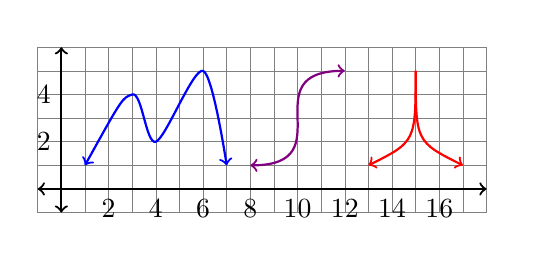
\begin{tikzpicture}[xscale=.3,yscale=.3]%[y=1cm,x=1cm]
               \draw[style = help lines, step=1cm] (-1,-1) grid (18,6);
               \foreach \x in {2,4,6,8,10,12,14,16}
                \draw (\x cm,1pt) -- (\x cm,-1pt) node[anchor=north] {$\x$};
               \foreach \y in {2,4}
                  \draw (1pt,\y cm) -- (-1pt,\y cm) node[anchor=east] {$\y$};
               \draw[thick,<->] (-1,0) -- (18,0) node[anchor=north west] {};%{x};
               \draw[thick,<->] (0,-1) -- (0,6) node[anchor=south east] {};%{y};
               \draw[blue,<->,thick] plot [smooth] coordinates {(1,1) (3,4) (4,2) (6,5) (7,1)};
               \draw[violet, thick,<->] (8,1) .. controls (12,1) and (8,5) .. (12,5);
               \draw[red, thick,<-] (13,1) .. controls (15,2) .. (15,5);
               \draw[red, thick,->] (15,5) .. controls (15,2) .. (17,1);     
            \end{tikzpicture}
        \end{column}  
      \end{columns} 
    \end{frame}
		\end{Verbatim}

	\subsection{Presentation Organization}
		Beamer includes several organizational tools for structuring your presentation. Using these tools produces a document with an extensive navigation system. Spend some time organizing your information before creating the content. A sample organizational scheme would be:
			\begin{enumerate}
				\item Title Page (including author and date)
				\item A table of contents frame (automatically generated by Beamer)
				\item Section delimiters (to separate topic sections)
				\item Subsection delimiters (to separate days spent within topic sections)
				\item Content to be displayed only during lectures (i.e. example solutions)
				\item Speaker (Teacher) notes not to be distributed to students
				\item Three formats (lecture presentation, student notes template for iPad, and printed student notes template)  
			\end{enumerate}
		Each of these ideas will be examined briefly below, but many more options are available. The Beamer User Guide referenced above contains almost 250 pages worth of customizations. 

		\subsubsection{Title Page}
		Putting the following in the preamble (before the  \verb|\begin{document}|  command) of your document and creating a plain title frame produces a title slide. Note that the date shown will reflect the date the presentation is created and will not update automatically.\\[.005in]
		\begin{minipage}[T]{.433\textwidth}
		\begin{Verbatim}
\title{Exponential and Logarithmic Functions} 
\author{Chapter 5}
\date{\today}

\begin{frame}[plain] 
	\titlepage
\end{frame}
		\end{Verbatim}
		\end{minipage}
		\begin{minipage}[T]{.433\textwidth}
		\includegraphics[scale=.15]{beamer/title_slide.png}
		\end{minipage}\\[.1in]
		Many more title frame options, such as subtitle, institution and a logo, can also be included.

		\subsubsection{Table of Contents}
		Assuming your frames are organized using \verb|\section| and \verb|\subsection| labels (see the next section), Beamer will generate a hyperlinked table of contents via \verb|\tableofcontents|.\\
		\begin{minipage}[T]{.5\textwidth}
		\begin{Verbatim}
\section*{Outline} 
\begin{frame}
	\tableofcontents	
\end{frame}
		\end{Verbatim}
		\end{minipage}
		\begin{minipage}[T]{.5\textwidth}
		\includegraphics[scale=.15]{beamer/toc.png}
		\end{minipage}\\[.1in]
		The star (*) after the section title will prevent that section from appearing in the table of contents. (Unfortunately, the starred section will still appear in the navigation links found in some themes.)

		\subsubsection{Section and Subsection}
		Organizing content with \verb|\section{title}| and \verb|\subsection{title}| puts hyperlinked titles into your presentation and table of contents. In the image below, both the section and subsection titles appear on the slide, as well as the frame title``Simplifying Expressions''. (The \verb|\label{}| and \verb|%fold| lines were added by my software.)\\[.1in]
		\begin{minipage}[h]{.5\textwidth}
		\begin{Verbatim}
\section[5.3 Logarithmic]{5.3 Logarithmic Functions} 
% (fold)
\label{sec:logarithmic_functions}
	\subsection{Day 1} % (fold)
	\label{sub:day_1}

		\end{Verbatim}
		\end{minipage}
		\begin{minipage}[T]{.5\textwidth}
		\includegraphics[scale=.15]{beamer/slide.png}
		\end{minipage}\\[.1in]
		The same content organization scheme also appears in \LaTeX \, documents which will be shown in Chapter \ref{sec:documents}. 
		
		\subsubsection{Hidden Content}
		Beamer includes a handout option which converts the digital pdf to a printable format. Included in the handout option is the ability to eliminate some information. For example, slides with answers or optional content (cartoons) can be excluded from the handout version by adding a \verb|<handout:0>| tag. \\
		
		\begin{minipage}[T]{.5\textwidth}
		\begin{Verbatim}
\begin{frame}<handout:0>[t]
	\begin{center}
		\includegraphics[scale=.5]{images/log_scale.png}
	\end{center}
\end{frame}

		\end{Verbatim}
		\end{minipage}
		\begin{minipage}[T]{.5\textwidth}
		\end{minipage}\\
		Combining the handout tag with the slide reveal numbering scheme produces a presentation that hides a solution until the presentation is advanced and does not include the solution in the handout version. For example, the slide below will have 5 versions. The first has no solution curves drawn while the second through fifth will each include one additional answer while keeping the previous answer(s). The \verb=<2-5|handout:0>= code below will show the $y=\log_{10} x$ graph (and its red dashed asymptote) on versions 2 though 5 of this slide. 

		\begin{Verbatim}
\draw<2-5|handout:0>[<->,thick,blue] plot[domain=.01:12,samples=100] (\x,{log10(\x)});
\draw<2-5|handout:0>[thick,red,dashed] (0,-3)--(0,-.5);
		\end{Verbatim}
		\begin{center}
		\includegraphics[scale=.2]{beamer/reveals.png}
		\end{center}

		Another way to separate content is to place a section inside a \verb|\only<beamer>{}| command. The included content will appear in the slideshow but not student handouts. 

		\subsubsection{Notes}
		Speaker or teacher notes can be embedded into a presentation by using the notes feature. Notes can be turned off when generating the student version by including \verb|{notes=hide}| in the Beamer \verb|\documentclass| options shown in section \ref{preamble}.\\[.1in]
		\begin{minipage}[T]{.5\textwidth}
		\begin{Verbatim}
\section*{notes} % (fold)
\label{sec:notes}
	\note {	add plots for log graphs in 5.3\\
			change asymptotes to red
			}	 
% section notes (end)
		\end{Verbatim}
		\end{minipage}
		\begin{minipage}[T]{.5\textwidth}
		\includegraphics[scale=.15]{beamer/notes.png}
	\end{minipage}\\[.1in]
		Chapter 19 of the Beamer user manual gives more details about the notes feature. 

		\subsubsection{Handouts}
		Once your slide presentation is complete, different versions can be generated depending on your audience. Four possibilities are:
			\begin{enumerate}
				\item Student iPad version
					\begin{itemize}
						\item suitable for use with Notability 
						\item no answers
					\end{itemize}
				\item Student printed version
					\begin{itemize}
						\item formatted to fit on 8.5x11 paper
						\item no answers
					\end{itemize}
				\item Lecture version
					\begin{itemize}
						\item includes answers and extra content
					\end{itemize}
				\item Teacher version
					\begin{itemize}
						\item includes teacher notes
					\end{itemize}
			\end{enumerate}
		One single .tex file contains the code to format the content into one of three different layouts.\\
		\begin{Verbatim}
%\documentclass[handout,aspectratio=169,mathserif,8pt,notes=hide]{beamer}%iPad
%****************Handout*******************
% \documentclass[handout,gray]{beamer}
% \usepackage{pgfpages}
% \usepackage[8pt]{extsizes}
% \pgfpagesuselayout{2 on 1}[a4paper,border shrink=1mm]
%****************HandoutEnd****************
%****Change to Cambridge theme*************
\documentclass[aspectratio=169,mathserif,8pt,xcolor=table,notes=show]{beamer}
		\end{Verbatim}
		The first line generates the iPad version (notice \verb|notes=hide|), the middle section generates a printable copy, and the last line produces the teacher/lecture slideshow version. Adding or removing the comment symbol (\%) determines which pdf is produced. (You may need to change themes for the printed version. )
	\subsection{Themes and Navigation}
		Many Beamer themes and color schemes are available. The navigation structure within a presentation depends on the theme chosen and whether titles, section and subsection labels have been used. Ian Blanes, an Associate Professor of Information and Communications in Barcelona has organized all of the theme and color possibilities at \href{http://deic.uab.es/~iblanes/beamer\_gallery/}{http://deic.uab.es/~iblanes/beamer\_gallery/}. (Many other Beamer theme and color matrices are available - search for ``Beamer theme matrix''.) Themes can be temporarily turned off by creating a slide with a \texttt{plain} style.

		\begin{Verbatim}
		\begin{frame}[plain]
			This is a plain white slide.
		\end{frame}
		\end{Verbatim}


% section beamer (end)
\section{Documents} % (fold)
\label{sec:documents}
	\subsection{Worksheets}
	\label{sub:worksheets}
	The process for creating a handout or worksheet begins with declaring a document type in the \verb|\documentclass{}| statement.\\
		\begin{minipage}[T]{.7\textwidth}
			\begin{Verbatim}
\documentclass[11pt]{article}
\usepackage{lipsum}%demo purposes only

\begin{document}

\title{A Document}
\author{Mr. Briody}
\date{\today}

\maketitle

\section{Introduction}
Solve this: $$\pi x^2-ex+i=0$$
\lipsum[2-4]
\end{document}
			\end{Verbatim}
		\end{minipage}
		\begin{minipage}[]{.3\textwidth}
			\includegraphics[scale=.25]{doc.png}
		\end{minipage}
		While the \verb|{article}| class may be useful for writing an article or a report, handouts and worksheets would probably benefit from a few modifications. Smaller margins and font size as well as a different title structure are needed. Changing to \verb|\documentclass{extarticle}| allows font sizes as small as 8 point. The \verb|geometry| package can change margin sizes and \verb|fancyhdr| puts information in headers and footers.\\
		\begin{minipage}[T]{.7\textwidth}
			\begin{Verbatim}
\documentclass[9pt]{extarticle}
\usepackage[margin=2cm]{geometry}
\usepackage{fancyhdr}
\usepackage{multicol}
\usepackage{lipsum}%demo purposes only

\newcommand{\thedate}{8/26/2014}
\newcommand{\theexam}{Candy Bar Contest}
\newcommand{\thecourse}{PreCalculus $\infty$ Briody}


\begin{document}

	\pagestyle{fancy}%headers and footers for all pages except first
		\lhead{\thecourse} \chead{\theexam} \rhead{\thedate}
		\lfoot{} \cfoot{\thepage} \rfoot{}


	\thispagestyle{plain}%first page setup
		\parindent 0ex
		\textbf{\thecourse} \hfill  \textbf{Name:}\makebox[6cm]{\hrulefill}

		\textbf{\theexam} \hfill \textbf{\thedate}


	\rule[1ex]{\textwidth}{.1pt} %horizontal line
	{\large {\bf Directions} }

		Do these correctly.\\[.5in]

	Content\\
	\begin{multicols}{2}
		\lipsum[1-3]
	\end{multicols}

	\newpage
	Second page content

\end{document}		
			\end{Verbatim}
		\end{minipage}
		\begin{minipage}[t]{.3\textwidth}
			\includegraphics[scale=.25]{wksht.png}
		\end{minipage}

		
	\subsection{Assessments}
		Two different assessment workflows will be presented. The first, \verb|\usepackage{exsheets}|, is a package that is incorporated within a \verb|\documentclass{extarticle}|. The second is a standalone document using \verb|\documentclass[10pt]{examdesign}|. Spending a little time configuring your document puts \LaTeX ~in charge of organization, formatting and numbering while the author can focus on content. Both methods can benefit from \LaTeX's powerful label and reference system which will be presented first. \\  
		\subsubsection{Detour: Labels and References}
		
		\begin{minipage}[T]{.65\textwidth}
		Adding \verb|\label{}| to a section, diagram or question produces a link within the document that can be called using \verb|\ref{}|. The internal link remains valid even if sections are rearranged or assessment questions are randomly ordered. For example, suppose the following ``intercept begin'' label is added to a question:
		\begin{Verbatim}
\begin{question}[class=easy]\label{intb}\addpoints{3}
		\end{Verbatim}
		Later, that question can be referenced using \verb|\ref{intb}| as in: 
		\begin{Verbatim}
What are the x-intercepts and y-intercepts for question \ref{intb}.
		\end{Verbatim}
		Output can be similar to that shown at right. If the questions are moved the value will update and virtual versions will have live hyperlinks. References are especially useful when the same directions or diagram are used for multiple questions. 
		\end{minipage}
		\begin{minipage}[]{.35\textwidth}
			\includegraphics[scale=.45]{ref.png}
		\end{minipage}

		\subsubsection{\texttt{exsheets} Package}
		Information about the \verb|exsheets| package can be found \href{https://ctan.org/pkg/exsheets?lang=en}{here} (\url{https://ctan.org/pkg/exsheets?lang=en}) and the full documentation pdf \href{http://ctan.mirrors.hoobly.com/macros/latex/contrib/exsheets/exsheets_en.pdf}{here} (\url{http://ctan.mirrors.hoobly.com/macros/latex/contrib/exsheets/exsheets_en.pdf}).  (You do not need to download the package - it is part of the standard \LaTeX ~distribution.) Two different examples using the \verb|exsheets| package will be shown. The first produces a typical assessment. Questions are spaced based on the teacher's estimate for the amount of space needed for student responses. Set-up requires a few lines of configuration code: 
		\begin{Verbatim}
\usepackage{exsheets}
\SetupExSheets{solution/print=false,question/name={},solution/name={}}	%Solutions on or off; 
\SetupExSheets{headings=runin}								% Puts questions next to number
\SetupExSheets{use-classes={easy,medium,hard}}					% Print questions by difficulty level
\SetupExSheets[points]{name=points}								% Puts questions next to number
\SetupExSheets{headings = margin-nr}
\newcommand*\pointsformat[1]{(#1) }
\SetupExSheets{points/format = \pointsformat}		
		\end{Verbatim}
		Headers and footers follow the same structure as shown in \ref{sub:worksheets}. A quiz question looks like...\\
		\begin{minipage}[]{.65\textwidth}
		\begin{Verbatim}
\begin{question}[class=easy]\addpoints{7} 
	If $f(x)=x^2-3$ find
	\begin{enumerate}
	 	\item $f(-2)$\\[0.3in]
	 	\item $f(a)$\\[0.3in]
	 	\item $f(x+h)$\\[0.3in]
	 \end{enumerate}  %\hfill  \makebox[1.3in]{\hrulefill}\\[1.5in]
\end{question}
\begin{solution}
\end{solution}
		\end{Verbatim}
		...which produces the question shown at right. If an answer blank is desired, uncomment by removing the \verb|%| near the \verb|\hfill|. Notice that question number (14 in this example) was never needed. \LaTeX ~handles the numbering. Also, \verb|exsheets| can print answers, either with the question or on a separate page, but if no answers are desired the solution \verb|\begin| and \verb|\end| are still required. 
		\end{minipage}
		\begin{minipage}[]{.35\textwidth}
			\includegraphics[scale=.45]{ques_ex1.png}
		\end{minipage}

		The second example presents all questions in a single grouping and student responses are submitted on separate blank paper. In addition, the top of the question page includes a scoring table. Code for the scoring table is shown below and the code for the entire document is in section \ref{sec:templates} (Templates).\\
		\begin{Verbatim}
\begin{center}
{\Large
\begin{tabular}{|l|*{\numberofquestions}{c|}c|}\hline
  Question & \ForEachQuestion{\GetQuestionProperty{counter}{#1}\iflastquestion{}{&}} & Total \\ \hline
  Points   & \ForEachQuestion{\GetQuestionProperty{points}{#1}\iflastquestion{}{&}} & \pointssum* \\ \hline
  Score  & \ForEachQuestion{\iflastquestion{}{&}} & \\ \hline
\end{tabular}
}
\end{center}
		\end{Verbatim}

			\includegraphics[scale=.45]{point_box.png}

			
		\subsubsection{\texttt{examdesign} Documentclass}	
		The second assessment example uses the \verb|examdesign| documentclass. Information, including sample documents can be found at \url{https://ctan.org/tex-archive/macros/latex/contrib/examdesign?lang=en} and documentation can be found at: \url{http://mirrors.concertpass.com/tex-archive/macros/latex/contrib/examdesign/examdesign.pdf}. Again, you do not need to download the class, but you may want to look at or download the three examples from the first website mentioned above.   

		The examdesign class includes predefined question types that can be included in one assessment. From the README file:
		\begin{Verbatim}
		* it allows for explicit markup of questions and answers;

		* the class will, at the user's request, automatically generate
		answer keys;

		* multiple versions of the same test can be generated
		automatically, with the ordering of questions within each section
		randomly permuted so as to minimize cheating;

		* the generated answer keys can be constructed either with or
		without the questions included;

		* environments are provided to assist in constructing the most
		common types of test question: matching, true/false,
		multiple-choice, fill-in-the-blank, and short answer/essay
		questions.
		 \end{Verbatim} 
		 Following a straightforward template, multiple choice assessments can be created and randomized (or not) with answer key(s) automatically generated. 
		 \begin{Verbatim}
 \NumberOfVersions{3}
 \setrandomseed{2019}
 \NoRearrange
		 \end{Verbatim}

		 A \verb|block| environment is used to surround questions that use the same set of directions or refer to the same graph. Questions within a block will not be randomly ordered, and \LaTeX's ~normal \verb|\label{}| and \verb|\ref{}|commands do not work, but are instead replaced by \verb|\thefirst| and \verb|\thelast|. An example block is shown below.

		\begin{minipage}[]{.6\textwidth}
			\begin{Verbatim}
\begin{block}[questions=2]
\hrulefill\\
For questions \thefirst \, and \thelast, $f'(x)=x\sin(x)-\cos(x)$ for $0<x<4$. Use your calculator.

\begin{question}
$f$ has a local maximum when $x$ is approximately
\choice {$0.9$}
\choice {$1.2$}
\choice {$2.3$}
\choice [!]{$3.4$}
\choice {$3.7$}
\end{question}

\begin{question}
$f$ has a point of inflection when $x$ is approximately
\choice {$0.9$}
\choice {$1.2$}
\choice [!]{$2.3$}
\choice {$3.4$}
\choice {$3.7$}
\end{question}
\hrule
\end{block}
			\end{Verbatim}
		\end{minipage}
		\begin{minipage}[]{.4\textwidth}
			\includegraphics[scale=.55]{block.png}
		\end{minipage}

		\subsubsection{Detour: Barcodes}
		Once your assessment has been created, the version can be hidden in a barcode using the \verb|makebarcode| package. In this example, the version is hidden in a string of seemingly random numbers and letters that can be revealed using any barcode scanner app. Use the code below as a starting point. The first line configures the package and is in the preamble while the second was placed at the end of the document in the \verb|\examclosing|.\\ 
		\begin{minipage}[t]{.6\textwidth}
			\begin{Verbatim}
\usepackage[code=Code39,X=.2mm,ratio=2.25,H=1cm]{makebarcode}
\barcode{3P\arabic{version}14159\Alph{version}2J\Roman{version}718281828}  		
			\end{Verbatim}
		\end{minipage}
		\begin{minipage}[t]{.4\textwidth}
		\includegraphics[scale=.6]{barcode.png}
		\end{minipage}

% section documents (end)

\section{Final Thoughts} % (fold)
\label{sec:final_thoughts}

Some final suggestions for getting comfortable with \LaTeX. 
\begin{enumerate}
	\item Code hunt: look for sample code. 
	\item Compile often.
	\item Comment out chunks of code (using command-option-/) to troubleshoot bugs. 
	\item Start small: create standalone diagrams or graphs.
	\item Make a simple document like a half-sheet daily quiz.
	\item Make a simple short presentation to go over homework or test prep.
	\item Don't try to include everything.  
	\item Google search "latex matrix" and get familiar with stackexchange.com. 

\end{enumerate}

% section final_thoughts (end)




\section{Templates} % (fold)
\label{sec:templates}

	\subsection{Standalone Formula}
		\begin{Verbatim}
\documentclass{standalone}

\begin{document}

$x=\frac{-b\pm\sqrt{b^2-4ac}}{2a}$

\end{document}		
		\end{Verbatim}
	\subsection{Standalone Graph}
		\begin{Verbatim}
\documentclass{standalone}
\usepackage{tikz}

\begin{document}

	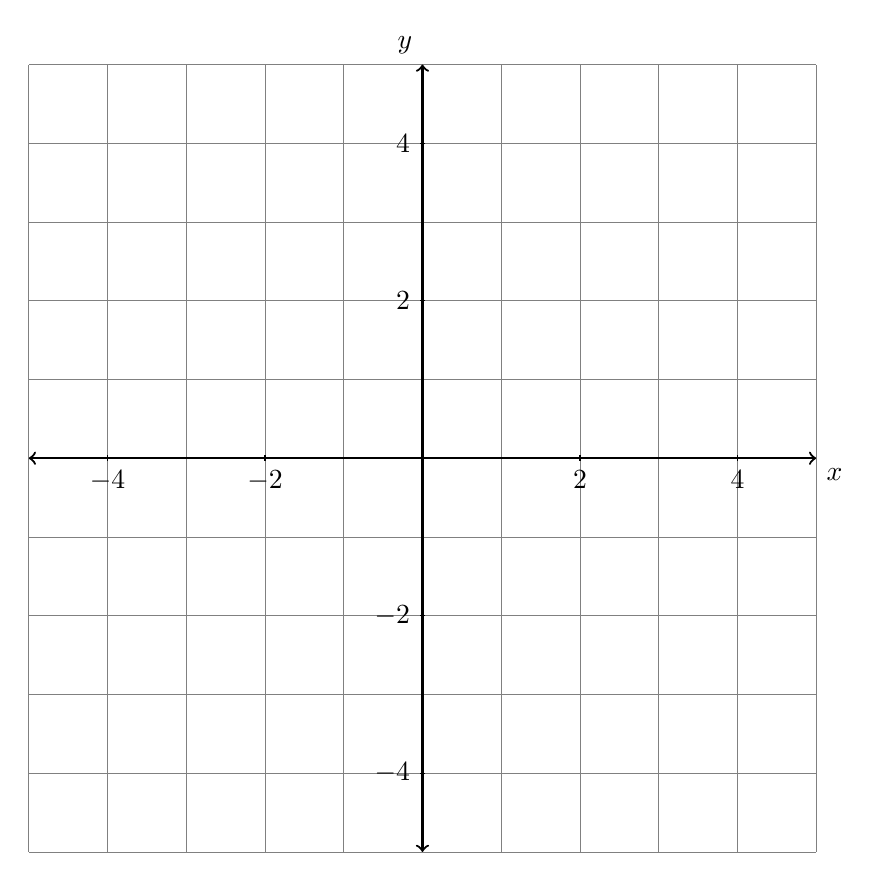
\begin{tikzpicture}[xscale=1,yscale=1]
		\draw[style = help lines, step=1cm] (-5,-5) grid (5,5);
		\draw[thick,<->] (-5,0) -- (5,0) node[anchor=north west] {$x$};
		\draw[thick,<->] (0,-5) -- (0,5) node[anchor=south east] {$y$};
		\foreach \x in {-4,-2,2,4}
		\draw (\x cm,1pt) -- (\x cm,-1pt) node[anchor=north] {$\x$};
		\foreach \y in {-4, -2, 2,4}
		\draw (1pt,\y cm) -- (-1pt,\y cm) node[anchor=east] {$\y$};
		%\draw[ultra thick,blue,<->] plot[domain=-3.89:3.75,samples=100] (\x,{.2*(\x+2)^2*(\x-3)});
		%\draw[ultra thick,blue,-] (-3,-4) -- (2,4);
		%\draw [red,ultra thick,domain=0:180] plot ({3*cos(\x)+2}, {3*sin(\x)});
		%\draw[ultra thick, blue,] (-2,-4) to [out=0, in=180] (4,1);
		%\draw[ultra thick, blue,] (0,-3)--(1,0)..controls (2.5,4) and (2.5,0)..(3,0)..controls (4.5,.9)..(6,3);
		%\draw [fill=black] (2,2)circle (3pt) node[above] {};
		%\draw [fill=white] (2,2)circle (3pt) node[above] {};
		%\foreach\x/\y/\z in {-1.8/1.2/P,-1/.3/Q,3.2/3.8/R,6.5/5/S,7.6/6/T}            
		   %  \draw [fill=black] (\x,\y)circle (3pt) node[above] {\z};
		%\node[draw=black,thick,fill=black!10,rounded corners=2pt] at (4,4) {Graph (d)};%LEGEND
	\end{tikzpicture}                     

\end{document}
		\end{Verbatim}

	\subsection{Beamer}
		\begin{Verbatim}
\documentclass[aspectratio=169,mathserif,8pt,notes=show]{beamer}
\usetheme{CambridgeUS} 
\usecolortheme{whale}
\usepackage{tikz}

\begin{document}

\begin{frame}[t]{Frame Title}
	\begin{columns}[T]
		\begin{column}{.433\textwidth}
			Column 1
		\end{column}	
		\begin{column}{.433\textwidth}
			Column 2
		\end{column}	
	\end{columns}	
\end{frame}

\end{document}
		\end{Verbatim}

	\subsection{Written Test}
		\begin{Verbatim}
\documentclass{extarticle}
	\usepackage{tikz}
	\usepackage[10pt]{extsizes}
	\usepackage[margin=1.3cm,headsep=0cm]{geometry}
	\usepackage{multicol}
	\usepackage{exsheets}
		\SetupExSheets{solution/print=false,question/name={},solution/name={}}	%Solutions on or off; 
		\SetupExSheets{headings=runin}								% Puts questions next to number
		\SetupExSheets{use-classes={easy,medium,hard}}					% Print questions by difficulty level
		\SetupExSheets[points]{name=points}								% Puts questions next to number
		\SetupExSheets{headings = margin-nr}
		\newcommand*\pointsformat[1]{(#1) }
		\SetupExSheets{points/format = \pointsformat}
	\usepackage{enumitem}				%Allow lists to be a, b, c and not 1, 2, 3
		\setenumerate[0]{label=(\alph*)}
	\usepackage{fancyhdr}
		\fancypagestyle{nocalc}{%Start of fancy page style
			\lhead{} \chead{{\bf \Large \calcnocalc}}	\rhead{ }
			\lfoot{} \cfoot{} \rfoot{}
		\renewcommand{\headrulewidth}{0pt} \renewcommand{\footrulewidth}{0pt}%removes unwanted header line
						}%end of fancy page style

		\newcommand{\thedate}{1/26/2019}
		\newcommand{\theexam}{Quiz 2.1 \& 2.2}
		\newcommand{\thecourse}{Math 101}
		\newcommand{\calcnocalc}{BABY CALCULATOR}

\begin{document}
\pagestyle{fancy}
\lhead{\thecourse} \chead{\theexam} \rhead{\thedate}
\lfoot{} \cfoot{\thepage} \rfoot{}				

\thispagestyle{nocalc}
\parindent 0ex
\textbf{\thecourse} \hfill  \textbf{Name:}
\makebox[6cm]{\hrulefill}\\
\textbf{\theexam} \hfill \textbf{\thedate}
						
\rule[1ex]{\textwidth}{.1pt}
{\large Please produce {\bf neat} and {\bf organized} solutions. Be sure to \framebox{box} your answers when appropriate. Messy or unsupported answers will receive no credit. If you would like additional paper please ask. Good luck.}\\
\rule[1ex]{\textwidth}{.1pt}

%%%%%%%%%%START TEST%%%%%%%%%%%%%%%
Directions: These questions will be in two columns.\\
\begin{minipage}[t]{.5\textwidth}
    \begin{question}[class=easy]\addpoints{3} 
    	Question 1\\  %\hfill \makebox[1.3in]{\hrulefill}\\[1.5in]
    \end{question}
    \begin{solution}
    \end{solution}
        
    \begin{question}[class=easy]\addpoints{2} 
        Question 2  %\hfill  \makebox[1.3in]{\hrulefill}\\[1.5in]
    \end{question}
    \begin{solution}
    \end{solution}
\end{minipage}%DO NOT put a blank line between
\begin{minipage}[t]{.5\textwidth}
    \begin{question}[class=easy]\addpoints{3} 
		Question 3\\  %\hfill \makebox[1.3in]{\hrulefill}\\[1.5in]
    \end{question}
    \begin{solution}
    \end{solution}
    
    \begin{question}[class=easy]\addpoints{3} 
        Question 4  %\hfill \makebox[1.3in]{\hrulefill}\\[1.5in]
        \begin{enumerate}
        \item first part\\[.5in]
        \item second part
        \end{enumerate}
    \end{question}
    \begin{solution}
    \end{solution}
\end{minipage}
\quad\\[1in]%newline
Directions: These questions will be in one columns.\\
\begin{question}[class=easy]\addpoints{3} 
        Question 5 with answer blank \hfill \makebox[1.3in]{\hrulefill}\\[1.5in]
\end{question}
\begin{solution}
\end{solution}
\newpage
\begin{question}[class=easy]\addpoints{3} 
    Question 6 with no answer blank %\hfill \makebox[1.3in]{\hrulefill}\\[1.5in]
\end{question}
\begin{solution}
\end{solution}

\newpage
Answers
\printsolutions
\end{document}	
		\end{Verbatim}
	\subsection{Written Test with Scoring Table}
		\begin{Verbatim}
\documentclass{extarticle}
	\usepackage{tikz}
	\usepackage[9pt]{extsizes}
	\usepackage[margin=1.3cm,headsep=0cm]{geometry}
	\usepackage{multicol}
	\usepackage{exsheets}
		\SetupExSheets{solution/print=false,question/name={},solution/name={}}	%Solutions on or off; 
		\SetupExSheets{headings=runin}								% Puts questions next to number
		\SetupExSheets{use-classes={easy,medium,hard}}					% Print questions by difficulty level
		\SetupExSheets[points]{name=pts.}								% Puts questions next to number
	\usepackage{microtype}
	\usepackage{comment} %comment out blocks
	\usepackage{fancyhdr}
\fancypagestyle{nocalc}{%Start of page style
	\lhead{} \chead{{\bf \Large NO CALCULATOR}}	\rhead{ }
	\lfoot{} \cfoot{} \rfoot{}
	\renewcommand{\headrulewidth}{0pt} \renewcommand{\footrulewidth}{0pt}
						} %end of page style
	%%%%%%%%%%%%%%%%%%%%%%%%%%%%%%
	% Change these appropriately.
	\newcommand{\thedate}{1/26/2019}
	\newcommand{\theexam}{Quiz \S1.3 Stuff and More Stuff}
	\newcommand{\thecourse}{PreCalculus $\infty$ Ms. Teacher}
	%%%%%%%%%%%%%%%%%%%%%%%%%%%%%%

\begin{document}
	\pagestyle{fancy}
	\lhead{\thecourse} \chead{\theexam} \rhead{\thedate}
	\lfoot{} \cfoot{\thepage} \rfoot{}
	\renewcommand{\headrulewidth}{0.4pt} \renewcommand{\footrulewidth}{0pt}
	\thispagestyle{nocalc}
	\parindent 0ex
	\textbf{\thecourse} \hfill  \textbf{Name:}
	\makebox[6cm]{\hrulefill}

	\textbf{\theexam} \hfill \textbf{\thedate}

	%Score Table
	\begin{center}
	{\Large
	\begin{tabular}{|l|*{\numberofquestions}{c|}c|}\hline
	%  Question & \ForEachQuestion{\QuestionNumber{#1}\iflastquestion{}{&}} & Total \\ \hline
	  Question & \ForEachQuestion{\GetQuestionProperty{counter}{#1}\iflastquestion{}{&}} & Total \\ \hline
	  Points   & \ForEachQuestion{\GetQuestionProperty{points}{#1}\iflastquestion{}{&}} & \pointssum* \\ \hline
	  Score  & \ForEachQuestion{\iflastquestion{}{&}} & \\ \hline
	\end{tabular}
	}
	\end{center}
	%%%%%%%%%%%%

\rule[1ex]{\textwidth}{.1pt}
{\large Please produce {\bf neat} and {\bf organized} solutions. Be sure to \framebox{box} your answers when appropriate. Messy or unsupported answers will receive no credit. If you would like scratch paper please ask. Good luck.}\\
\rule[1ex]{\textwidth}{.1pt}

%%%%%%%%%%%%%%%%%%QUESTIONS%%%%%%%%%%%%%%%%%%%%%%
\begin{question}[class=medium]\addpoints*{2}
Find the domain of $f(x)=\frac{1}{x-2}$. 
\end{question}
\begin{solution}
$(-\infty,2)(2,\infty)$
\end{solution}

\begin{question}[class=medium]\addpoints*{4}
Find the domain and range of $g(x)=\sqrt{2-x}+2$.
\end{question}
\begin{solution}
Domain: $(-\infty,3)$ Range:$[3,\infty]$
\end{solution}

\begin{question}[class=medium]\addbonus*{3}
{\textbf EC} Find the domain of $h(x)=\frac{1}{x-4}+\sqrt{x}$.
\end{question}
\begin{solution}
$[0,4)\cup(4,\infty)$ 
\end{solution}
%%%%%%%%%%%%%%%%%%QUESTIONS%%%%%%%%%%%%%%%%%%%%%%
\newpage
Answers 
\printsolutions
\end{document}		
		\end{Verbatim}

	\subsection{Multiple Choice Test}
\begin{Verbatim}
\documentclass[10pt]{examdesign}
\usepackage{amsmath}
\usepackage{tikz,adjustbox}
  \usetikzlibrary{arrows}
\usepackage{multicol}
\usepackage{blindtext}
\usepackage{float}%force table to stay with question
\SectionFont{\large\sffamily}
\Fullpages
\ContinuousNumbering
\ShortKey
\DefineAnswerWrapper{}{}
\NumberOfVersions{3}
%\IncludeFromFile{foobar.tex}

\class{Multiple Choice Test}

\begin{examtop}
  \noindent Name:\rule{3.8in}{.4pt}
  \begin{center}
    \textbf{Math 101} \\
    \textbf{\classdata}\\% \Alph{version}} \\
    \textbf{January, 2019}\\
    Each question has {\bf one} best answer. {\bf NO CALCULATOR} needed.\\
    Version \Alph{version}
  \end{center}
\end{examtop}

\begin{keytop}
  \classdata \quad Version: \Alph{version}
\end{keytop}

\setrandomseed{2019}
\NoRearrange %comment out to randomize

\begin{document}
\begin{multiplechoice}[resetcounter=no,keycolumns=3,suppressprefix=yes,examcolumns=2]

\begin{question}
$\int\limits_{1}^2\frac{dz}{3-z}=$
\choice {$-\ln2$}
\choice {$\frac{3}{4}$}
\choice {$2\left(\sqrt{2}-1\right)$}
\choice {$\frac{1}{2}\ln2$}
\choice [!]{$\ln2$}
\end{question}

\begin{question}
The integral $\int\limits_{-4}^4\sqrt{16-x^2}\,dx$ gives the area of
\choice {a cricle of radius $4$}
\choice [!]{a semicircle of radius $4$}
\choice {a quadrant of a circle of radius $4$}
\choice {an ellipse whose semi-major axis is $4$}
\choice {none of these}
\end{question}

\begin{examclosing}
  \vfill
    End of Exam. 
\end{examclosing}

\end{multiplechoice}
\end{document}
\end{Verbatim}

	\subsection{Others}
	\begin{itemize}
	\item Document templates can be found at: \url{http://www.latextemplates.com/}
	\item The \texttt{TikZ} gallery is at \url{http://www.texample.net/tikz/examples/}; look for the \textbf{Mathematics} link in the \textbf{Scientific and technical areas} section.
	\end{itemize}
% section templates (end)	

	\end{document}